\begin{figure}[htbp]
	\centering
	\resizebox{0.8\textwidth}{!}{%
		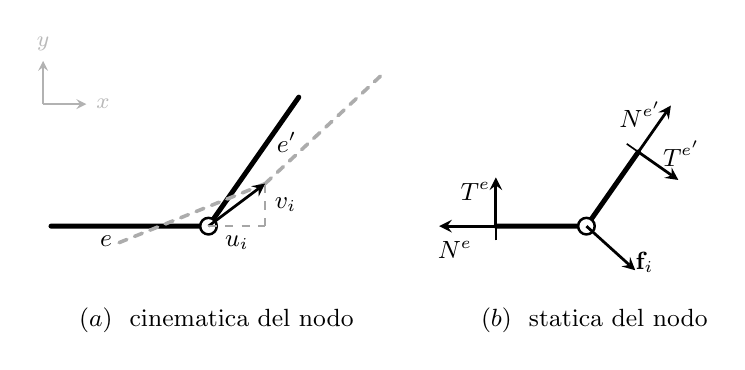
\begin{tikzpicture}[
			trave/.style={line width=1.8pt, line cap=round, line join=round, black},
			ghost/.style={line width=1.3pt, dashed, line cap=round, line join=round, gray!65},
			forza/.style={->, >=stealth, line width=1.0pt, black},
			momento/.style={->, >=stealth, line width=0.9pt, black},
			guida/.style={line width=0.55pt, dashed, gray!70},
			taglio/.style={line width=0.6pt, black},
			asse/.style={->, >=stealth, line width=0.6pt, gray!60},
			cerniera/.style={circle, draw=black, fill=white, line width=0.9pt, inner sep=0pt, minimum size=6pt},
			lab/.style={font=\small},
			labg/.style={font=\footnotesize, gray!55},
			]
			
			\def\Le{2.0}      % trave e (orizzontale, a sinistra del nodo)
			\def\Lep{2.0}     % trave e'
			\def\ang{55}      % inclinazione di e'  (angolo incluso ~125°)
			\def\SEP{4.8}     % separazione tra i pannelli
			
			%%═══ PANNELLO (a) — cinematica del nodo ══════════════════════════
			\begin{scope}
				% configurazione indeformata
				\draw[trave] (-\Le,0) -- (0,0) -- ({\Lep*cos(\ang)},{\Lep*sin(\ang)});
				% traslazione CONDIVISA, rotazioni INDIPENDENTI
				\def\du{0.72}\def\dv{0.54}
				\def\rote{22}     % rotazione trave e
				\def\rotep{-12}   % rotazione trave e' (diversa: la cerniera lascia libera la rotazione relativa)
				% configurazione spostata: nodo traslato, ogni trave ruotata per conto proprio attorno al nodo
				\begin{scope}[shift={(\du,\dv)}]
					\draw[ghost, rotate=\rote]  (-\Le,0) -- (0,0);
					\draw[ghost, rotate=\rotep] (0,0) -- ({\Lep*cos(\ang)},{\Lep*sin(\ang)});
				\end{scope}
				% cerniera al nodo (configurazione di riferimento)
				\node[cerniera] at (0,0) {};
				% spostamento nodale condiviso e componenti nel riferimento globale
				\draw[forza] (0,0) -- (\du,\dv);
				\draw[guida] (0,0) -- (\du,0);
				\draw[guida] (\du,0) -- (\du,\dv);
				\node[lab, below] at ({\du/2},0) {$u_i$};
				\node[lab, right] at (\du,{\dv/2}) {$v_i$};
				% rotazioni indipendenti — archi simbolici al nodo traslato  [POSIZIONI DA RIFINIRE]
				%				\draw[momento, line width=1.0pt] ({\du+0.42*cos(150)},{\dv+0.42*sin(150)}) arc (150:205:0.42);
				%				\node[lab] at ({\du-0.42},{\dv+0.50}) {$\vartheta_e$};
				%				\draw[momento, line width=1.0pt] ({\du+0.46*cos(82)},{\dv+0.46*sin(82)}) arc (82:37:0.46);
				%				\node[lab] at ({\du+0.42},{\dv+0.68}) {$\vartheta_{e'}$};
				% etichette travi
				\node[lab, below] at (-1.30,0) {$e$};
				\node[lab, right] at ({1.30*cos(\ang)},{1.30*sin(\ang)}) {$e'$};
				% assi globali
				\begin{scope}[shift={(-\Le-0.10,1.55)}]
					\draw[asse] (0,0) -- (0.55,0) node[labg, right] {$x$};
					\draw[asse] (0,0) -- (0,0.55) node[labg, above] {$y$};
				\end{scope}
				\node[lab] at (0.10,-1.20) {$(a)$ \ cinematica del nodo};
			\end{scope}
			
			%%═══ PANNELLO (b) — statica del nodo (corpo libero) ══════════════
			\begin{scope}[xshift=\SEP cm]
				\def\dc{1.15}   % posizione del taglio lungo ciascuna trave
				% tronconi isolati delle due travi
				\draw[trave] (-\dc,0) -- (0,0) -- ({\dc*cos(\ang)},{\dc*sin(\ang)});
				% cerniera al nodo (perno)
				\node[cerniera] at (0,0) {};
				
				% ---- estremità della trave e (taglio a sinistra): trasmette N, T; M = 0 ----
				\draw[taglio] (-\dc,-0.18) -- (-\dc,0.18);            % sezione
				\draw[forza]  (-\dc,0) -- (-\dc-0.72,0);              % N_e (trazione, uscente)
				\node[lab] at (-\dc-0.52,-0.30) {$N^e$};
				\draw[forza]  (-\dc,0) -- (-\dc,0.62);                % T_e (trasversale, verso l'alto)
				\node[lab] at (-\dc-0.26,0.44) {$T^e$};
				
				% ---- estremità della trave e' (taglio in alto a destra): trasmette N, T; M = 0 ----
				\begin{scope}[shift={({\dc*cos(\ang)},{\dc*sin(\ang)})}, rotate=\ang]
					\draw[taglio] (0,-0.18) -- (0,0.18);              % sezione
					\draw[forza]  (0,0) -- (0.72,0);                  % N_{e'} (trazione, uscente)
					\node[lab] at (0.40,0.25) {$N^{e'}$};
					\draw[forza]  (0,0) -- (0,-0.62);                 % T_{e'} (invertito)
					\node[lab] at (0.30,-0.46) {$T^{e'}$};
				\end{scope}
				
				% carico nodale esterno (eventuale): sola forza f_i
				% (una coppia concentrata non è trasmessa dalla cerniera: cfr. nota nel testo)
				\draw[forza] (0,0) -- (0.62,-0.56);
				\node[lab, right] at (0.50,-0.46) {$\mathbf{f}_i$};
				
				\node[lab] at (0.10,-1.20) {$(b)$ \ statica del nodo};
			\end{scope}
			
		\end{tikzpicture}
	}%
	\caption{Cerniera interna tra due travi, $e$ ed $e'$. A sinistra:
		cinematica del nodo --- le traslazioni $(u_i, v_i)$ nel
		riferimento globale sono condivise da entrambe le travi,
		mentre le rotazioni $\vartheta^e$ e $\vartheta^{e'}$ restano
		indipendenti: l'angolo tra le travi non si conserva.
		A destra: statica del nodo isolato come corpo libero ---
		ciascuna trave trasmette le sole caratteristiche di forza
		$N$ e $T$ nel rispettivo sistema locale, mentre il momento
		non è trasmesso ($M = 0$ su ciascun elemento); con
		l'eventuale carico nodale $\mathbf{f}_i$, l'equilibrio del
		nodo si riduce a $\sum\mathbf{f}=\mathbf{0}$ --- due
		equazioni scalari, una in meno del nodo rigido.}
	\label{fig:cerniera_interna}
\end{figure}
